\documentclass[10pt,a4paper]{report}

\usepackage[utf8]{inputenc}
\usepackage{amsmath}
\usepackage{amsfonts}
\usepackage{amssymb}
\usepackage{graphicx}
\usepackage{color}
\usepackage{enumitem}
\usepackage[top=1cm, bottom=2cm, left=2cm, right=2cm]{geometry}

\usepackage{fancyhdr}
\pagestyle{fancy}

\fancyhead{}
\fancyfoot{} 
\lhead{
\includegraphics{../Logo/logoKNKMini.jpg} \hspace{0.1cm} Kould Not Konect  \hspace{0.4cm} \vline}
\chead{Document de Conception Générale}
\rhead{Kould Not Share}
\rfoot{\thepage}

\author{Kevin BASCOL, Kevin LAOUSSING, Nicolas REYNAUD}
\title{Document de conception générale}
\date{3 Novembre 2014}

\makeatletter
\renewcommand{\thesection}{\@arabic\c@section}
\makeatother

\begin{document}

\makeatletter
	\begin{titlepage}
	
	\begin{figure}
		\begin{minipage}[c]{.46\linewidth}
		\end{minipage} \hfill
		\begin{minipage}[c]{.20\linewidth}
			\begin{center}
				
\includegraphics{../Logo/logoKNK.jpg}\\
				{\large Kould Not Konect}
			\end{center}
		\end{minipage}
	\vspace{1cm}
	\end{figure}
	
	\centering
		{
		\hrule height 2pt
		\vspace{0.7cm}
		\Huge \textbf{\@title}}\\
		\vspace{0.7cm}
		\hrule height 2pt
		\vspace{1.5cm}
		{\LARGE  Projet \textbf{Kould Not Share} v1.0}
		
		\vfill
		
		\begin{tabular}{|c|c|c|}
			\hline
			Version & Date & Description\\
			\hline
			V.1 & 16/11/14 & Première version de la conception générale\\
			\hline
			 & & \\
			\hline
			 & & \\
			\hline
		\end{tabular}\\
		\vspace{1cm}
		\@author\\
		\end{titlepage}
\makeatother
\setcounter{secnumdepth}{5}
\setcounter{tocdepth}{5}
\renewcommand{\contentsname}{Sommaire}
\begingroup\makeatletter
\def\@makeschapterhead#1{%
  {\parindent \z@ \raggedright
    \normalfont
    \interlinepenalty\@M
    \Huge \bfseries  #1\par\nobreak
    \vskip 20pt% <---- à réduire pour avoir plus de place
  }}\makeatother
\tableofcontents
\endgroup
\thispagestyle{empty}
\setcounter{page}{0}
\newpage

\newgeometry{top=2cm, bottom=2cm, left=2cm, right=2cm}



\section{Objectif du document}
\begin{flushleft}
Ce document présente la conception logicielles et matérielles de la version 1.0 du projet Kould Not Share de l'entreprise Kould Not Konnect. Les responsables de ce projet sont Nicolas Reynaud, Kevin Laoussing et Kevin Bascol.
\end{flushleft}

\section{Architecture du système Kould Not Share}

	\subsection{Architecture MVC}
		\begin{flushleft}
		Notre système Kould Not Share est composé en deux sous-système : le client et le serveur. Chacun de ces sous-systèmes utilisent un patron modèle-vue-controleur (MVC).\\
Ce patron permettra de bien séparer les données, la présentation et les traitements qui correspond respectivement aux trois parties suivantes :le modèle, la vue et le contrôleur (voir section 2.1 Schéma du système).\\
Pour rappel, lorsqu'un utilisateur interagie avec l'interface graphique de l'application (qui correspond à la vue du patron MVC), celle-ci envoie une requête  :
			\begin{itemize}
				\item la requête envoyée depuis la vue est analysée par le contrôleur (par exemple un clic de souris pour lancer un traitement de données) ;
    			\item le contrôleur demande au modèle approprié d'effectuer les traitements et notifie à la vue que la requête est traitée ;
    			\item la vue notifiée fait une requête au modèle pour se mettre à jour (par exemple affiche le résultat du traitement "via" le modèle).

			\end{itemize}
		\textbf{Remarque : }L'implémentation du patron MVC, utilise un autre patron de conception : Observateur.\\
D'après le patron de conception observateur, la vue est un " observateur " du modèle qui est lui " observable ".
		\end{flushleft}
    

	\subsection{Architecture modulaire du système}

		\subsubsection{Schéma de la décomposition modulaire du système}
			\begin{flushleft}
			Ce schéma présente d'une part le patron utilisé par le système et d'autre part la décomposition modulaire du système.\\
			Il décrit de manière général le fonctionnement du système à travers les interaction entre les modules.
			\end{flushleft}
			\begin{center}
				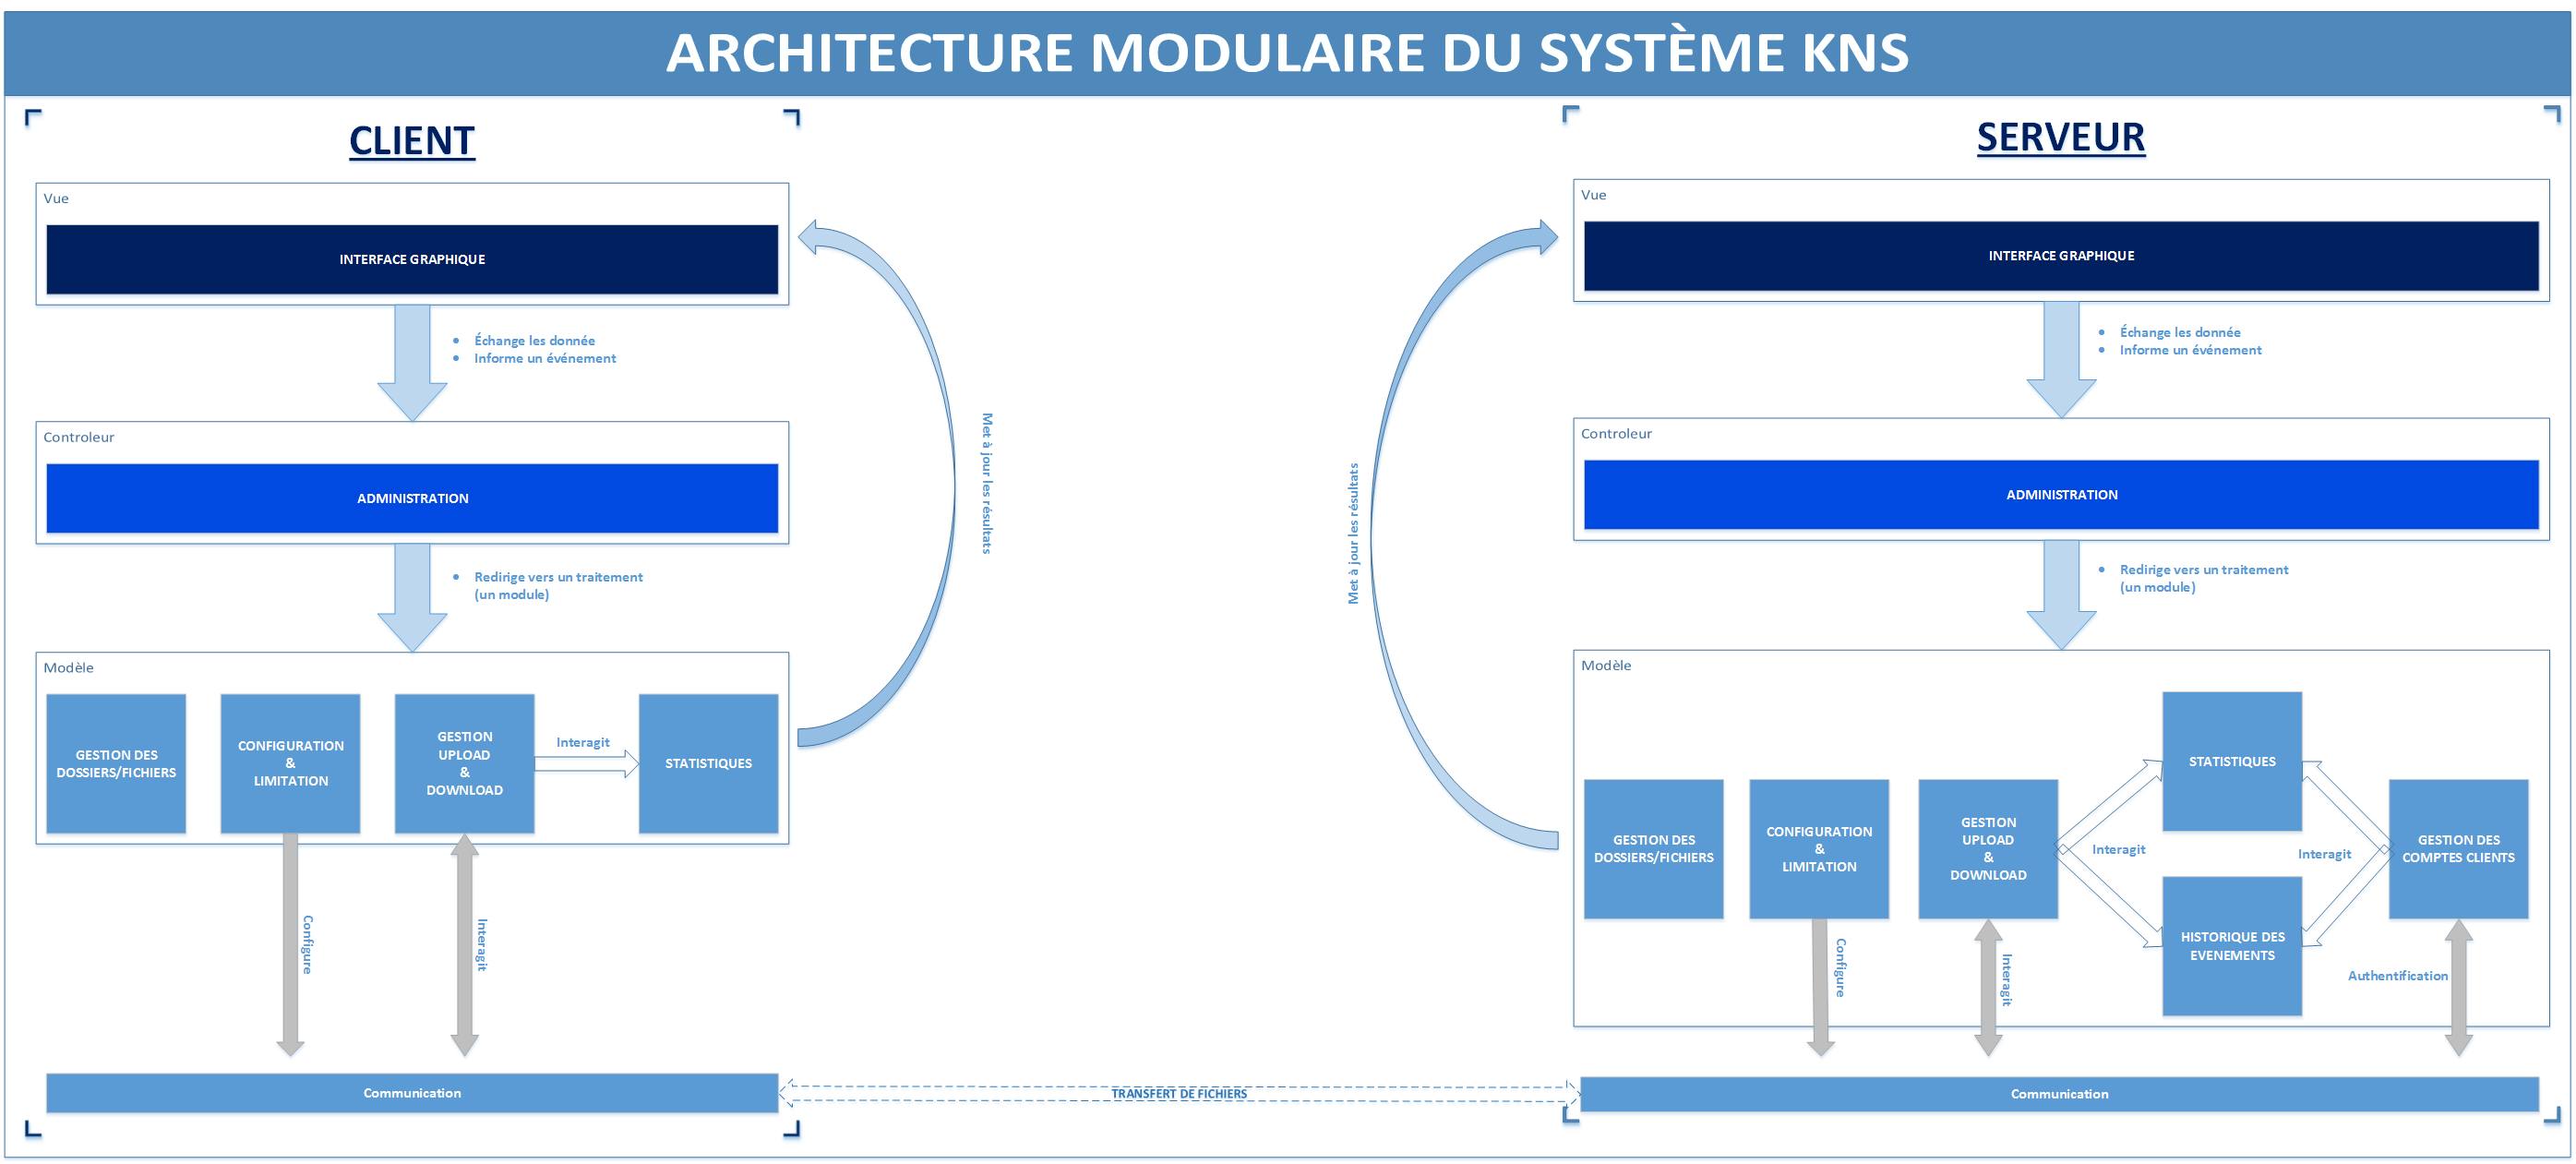
\includegraphics[scale=0.23]{Ressources/modules_KNS.png}
			\end{center}
		(cf Annexe.)

\newpage
		\subsubsection{Description des modules}
	
			\paragraph{Modules Client}

				\subparagraph{Module interface graphique}
				\begin{flushleft}
				Ce module contiendra toutes les classes Java en rapport avec l'interface graphique du client KNS. Ce module correspond aussi à la vue du patron MVC, il doit par conséquent accomplir les tâches suivantes :\\
					
					\begin{itemize}
						\item Présenter les résultats renvoyés par le modèle.
						\item Recevoir toute action de l'utilisateur (hover, clic de souris, sélection d'un bouton radio, cochage d'une case, entrée de texte, de mouvements, de voix, etc.).
						\item Envoyer ces différents événements au contrôleur. 
					\end{itemize}
					
					\textbf{Ce module n'effectue pas de traitement, elle se contente d'afficher les résultats des traitements effectués par le modèle et d'interagir avec l'utilisateur.}\\
				\end{flushleft}
						
				\subparagraph{Module d'administration}
				
				\begin{flushleft}
				Techniquement, le module d'administration est une implémentation du contrôleur du patron MVC, il doit donc contenir toutes les classes permettant d'accomplir les tâches spécifiques d'un contrôleur :
				
				\begin{itemize}
					\item Prendre en charge la gestion des événements de synchronisation pour mettre à jour la vue ou le modèle et les synchroniser. 
					\item Recevoir tous les événements de la vue et enclencher les actions à effectuer. 
					\item Si une action nécessite un changement des données, faire une demande de modification des données au modèle afin que les données affichées se mettent à jour. 
				\end{itemize}
				
Ce module n'effectue aucun traitement, ni de modification sur la donnée. Il analyse la requête du client (envoyé depuis la vue) et se contente d'appeler le modèle adéquat et de renvoyer la vue correspondant à la demande.\\
Le seul traitement du contrôleur est de déterminer l'origine de chaque événement. Ce tri des événements pourrait-être implémenter par le patron de conception Stratégie.
				\end{flushleft}
				
	
				\subparagraph{Module de gestion des dossiers}
				\begin{flushleft}
				Ce module appartient à la partie modèle du patron MVC. Le module de gestion regroupe  toutes les classes en rapport avec la gestion des dossiers. L'ensemble de ces classes réalisent les traitements tel que la création d'un répertoire, la suppression de fichiers... (cf Document des spécifications des exigences).\\ 
				\end{flushleft}
	
				\subparagraph{Module de configuration et limitation}	
				\begin{flushleft}
				Ce module appartient à la partie modèle du patron MVC. Le module de configuration et limitation regroupe toutes les classes qui réalisent les configurations du client et les limitations des transferts de fichiers du module de communication.
				\end{flushleft}
	
				\subparagraph{Module de upload/download}
				\begin{flushleft}
				Ce module appartient à la partie modèle du patron MVC. Le module de upload/download regroupe toutes les classes qui réalisent les opérations d'upload et de download d'un fichier. Pour chacun de ces opérations le module interagit avec le module de communication effectuer le transfert de fichiers, et le module de statistique pour comptabiliser les transferts. (cf Document des spécifications des exigences).
				\end{flushleft}
	
				\subparagraph{Module de statistiques}
				\begin{flushleft}
				Ce module appartient à la partie modèle du patron MVC. Le module de statistique regroupe toutes les classes qui réalisent les opérations en rapport avec les graphes. Ce moule interagi avec le module d'upload et de download, pour comptabiliser les transferts. Le module de statistique gere toutes les statistiques ainsi que le stockages de celle ci.
				\end{flushleft}
				
				\subparagraph{Module de communication}

\newpage
			\paragraph{Modules Serveur}

				\subparagraph{Module de l'interface graphique}
				\begin{flushleft}
				Ce module contiendra toutes les classes Java en rapport avec l'interface graphique du client KNS. Ce module correspond aussi à la vue du patron MVC, il doit par conséquent accomplir les tâches suivantes :\\
					
					\begin{itemize}
						\item Présenter les résultats renvoyés par le modèle.
						\item Recevoir toute action de l'utilisateur (hover, clic de souris, sélection d'un bouton radio, cochage d'une case, entrée de texte, de mouvements, de voix, etc.).
						\item Envoyer ces différents événements au contrôleur. 
					\end{itemize}
					
					\textbf{Ce module n'effectue pas de traitement, elle se contente d'afficher les résultats des traitements effectués par le modèle et d'interagir avec l'utilisateur.}\\
				\end{flushleft}
				
				\subparagraph{Module d'administration}
				\begin{flushleft}
				Techniquement, le module d'administration est une implémentation du contrôleur du patron MVC, il doit donc contenir toutes les classes permettant d'accomplir les tâches spécifiques d'un contrôleur :
				
				\begin{itemize}
					\item Prendre en charge la gestion des événements de synchronisation pour mettre à jour la vue ou le modèle et les synchroniser. 
					\item Recevoir tous les événements de la vue et enclencher les actions à effectuer. 
					\item Si une action nécessite un changement des données, faire une demande de modification des données au modèle afin que les données affichées se mettent à jour. 
				\end{itemize}
				
Ce module n'effectue aucun traitement, ni de modification sur la donnée. Il analyse la requête du client (envoyé depuis la vue) et se contente d'appeler le modèle adéquat et de renvoyer la vue correspondant à la demande.\\
Le seul traitement du contrôleur est de déterminer l'origine de chaque événement. Ce tri des événements pourrait-être implémenter par le patron de conception Stratégie.
				\end{flushleft}
	
				\subparagraph{Module de gestion des dossiers}
				\begin{flushleft}
				Ce module appartient à la partie modèle du patron MVC. Le module de gestion regroupe  toutes les classes en rapport avec la gestion des dossiers. L'ensemble de ces classes réalisent les traitements tel que la création d'un répertoire, la suppression de fichiers... (cf Document des spécifications des exigences).\\ 
				\end{flushleft}
	
				\subparagraph{Module de configuration et limitation}	
				\begin{flushleft}
				Ce module appartient à la partie modèle du patron MVC. Le module de configuration et limitation regroupe toutes les classes qui réalisent les configurations du serveur et les limitations des transferts de fichiers du module de communication.
				\end{flushleft}
	
				\subparagraph{Module de statistiques}
				\begin{flushleft}
				Ce module appartient à la partie modèle du patron MVC. Le module de statistique regroupe toutes les classes qui réalisent les opérations en rapport avec les graphes. Ce moule interagi avec le module d'upload et de download, pour comptabiliser les transferts. Le module de statistique gere toutes les statistiques ainsi que le stockages de celle ci.
				\end{flushleft}
				
	
				\subparagraph{Module des historiques des événements}
	
	
				\subparagraph{Module de gestion des comptes clients}
	
	
				\subparagraph{Module de communication}

\section{Définition des principales structures de données}

	\subsection{Structures de données}

	\subsection{Interactions entre les structures de données} %<--- diagramme de séquence ?%

\newpage
\section{Annexe}

\subsection{Architecture modulaire du système KNS}
	\begin{center}
	\rotatebox{270}{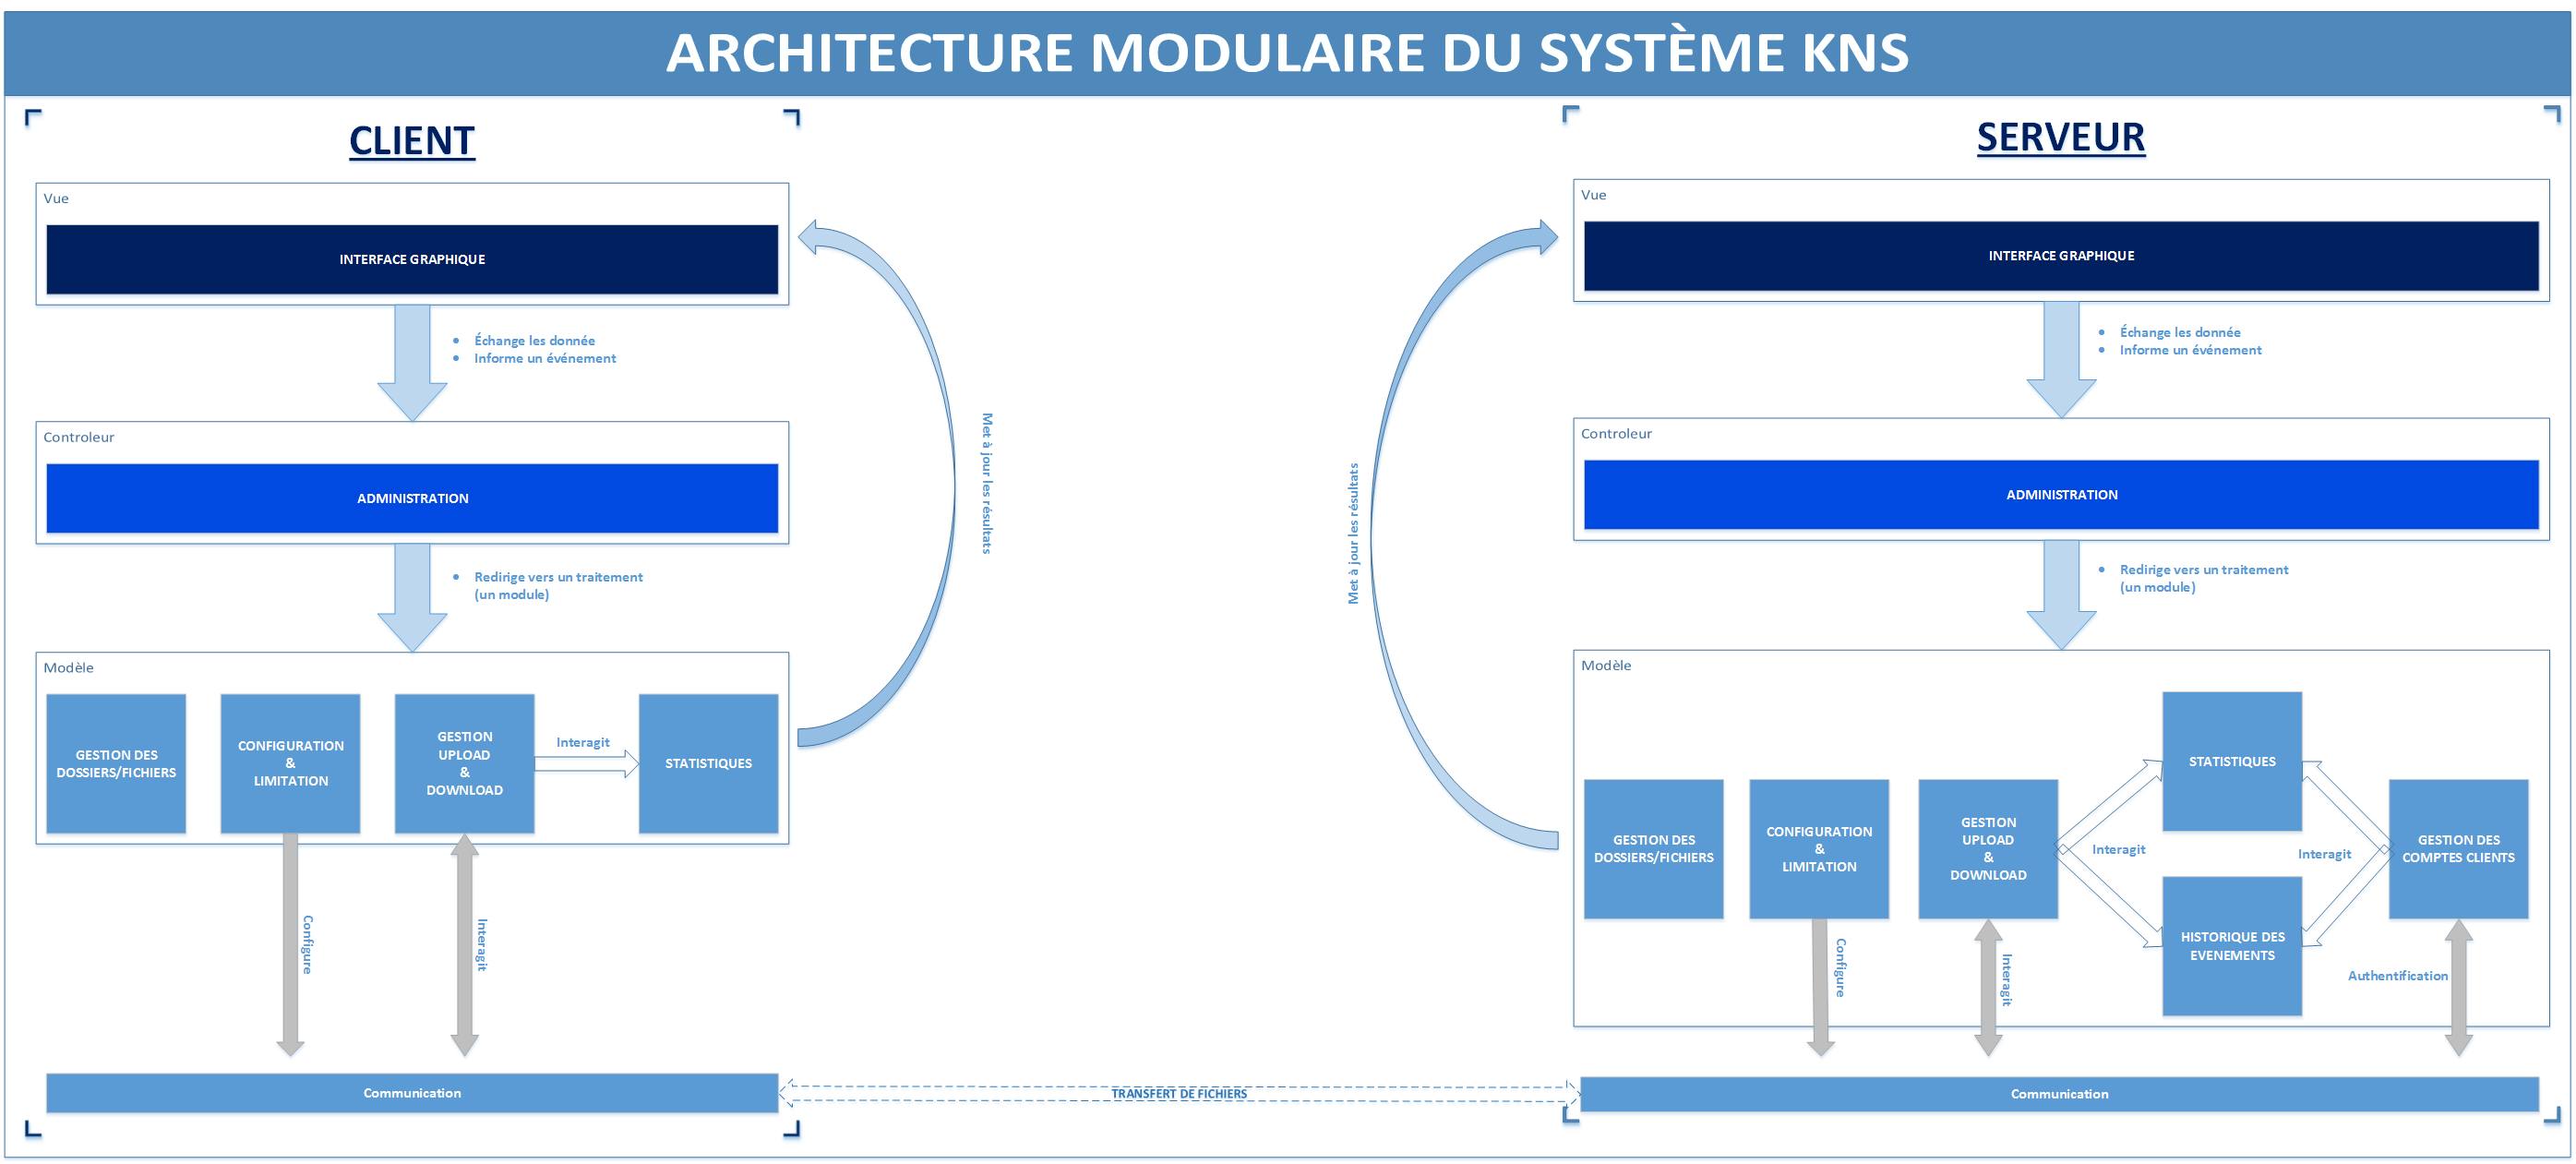
\includegraphics[scale=0.35]{Ressources/modules_KNS.png}}	
	\end{center}
\end{document}